\documentclass[Ex4_Zusammenfassung.tex]{subfiles}

\begin{document}
\section{Isospin}
\textbf{von \michi \& \paul}\\

Isospin ist ein theoretisches Konzept, andere Art der Beschreibung.
\subsection{Grundidee}
\begin{itemize}
	\item up--, down--Quarks sind sehr ähnlich; sie haben das gleiche Verhalten unter starker Wechselwirkung, $\approx$ gleiche Masse (andere Quarks haben deutlich unterschiedlichere Massen).
	\item up--, down--Quarks unterscheiden sich nur in ihrer Ladung $\lp - \nicefrac{1}{3}e\rp,\ \lp \nicefrac{2}{3}e \rp $
	\item Mann kann sie als ein Teilchen beschreiben, das sich lediglich in unterschiedlichen Zuständen befindet.
	\item Wir kennen dies bereits von $e^-$: \\
	Elektronen sind Teilchensorte, können aber in zwei verschiedenen Zuständen auftreten: spin up $(\uparrow)$ und spin down $(\downarrow)$.
	\item Analog können wir diese Anschauung des ''1. Generation--Quarks'' mit Quantenzahlen versehen. Wir finden, dass diese die gleichen algebraischen Eigenschaften wie der Spin haben, deshalb nennt man sie ''Isospinquantenzahlen'' (Wortbedeutung ''Iso'': ''quantitativ gleich zu''). Diese Analogie ist jedoch \textbf{nur} mathematischer Natur! Physikalisch hat der Spin nichts mit Drehimpulsen und magnetischen Momenten zu tun, wie es beim (echten) Spin der Fall ist. 
\end{itemize}

\subsection{Grafische Veranschaulichung der Analogie}
\begin{figure}[H]
	\centering
	\begin{tikzpicture}
		%nodes 
			%gen1
		\node at (0,0.5) (gen1) [text width=2.5cm] {''Quarks der 1. Generation''};
		\node at (0,-0.3) (updown) {$\kern 1em \ket{\text{up}} \qquad \ket{\text{down}}$};
		\node at (0,-0.8) (genI3) {$\kern 0.4em I_3 = \nicefrac{1}{2} \quad I_3 = -\nicefrac{1}{2}$};
			%elek.
		\node at (6,0.7) (elek) {Elektronen};
		\node at (6,-0.1) (ud) {$\ket{\uparrow} \qquad \ket{\downarrow}$};
		\node at (6,-0.7) (ms) {$\kern 0.4em m_S = \nicefrac{1}{2} \quad m_S = -\nicefrac{1}{2}$};
			%nukleonen
		\node at (0,-3.8) (nuk) {Nukleonen};
		\node at (0,-4.6) (pn) {$\kern 0.7em \ket{\text{Proton}} \quad \ket{\text{Neutron}}$};
		\node at (0,-5.2) (nukI3) {$\kern 0.4em I_3 = \nicefrac{1}{2} \quad I_3 = -\nicefrac{1}{2}$};
			%equiv sign
		\node at (3,0) (sign) [scale=3]{$\hat{=}$};
		
		%lines
		\draw [dashed] (gen1.south) -- (0,-1.5);
		\draw [dashed] (elek.south) -- (6,-1.5);
		\draw [dashed] (nuk.south) -- (0,-6);
		
		%shapes
		\draw (0,0) ellipse (2.2cm and 1.5cm);
		\draw (6,0) ellipse (2.2cm and 1.5cm);
		\draw (0,-4.5) ellipse (2.2cm and 1.5cm);
		
		%arrows
		\draw [blue, thick, >=stealth'] (-2, -1) edge [bend right, ->] node [midway, left, text width=0.8cm] {oder auch:} (-2, -3.5);
		
		%braces
		\draw [decoration={brace}, decorate, line width=1pt, red] (-2.2,1.7) -- (2.2,1.7) node [pos=0.5, above, yshift=2pt] {$I=\nicefrac{1}{2}$};
		\draw [decoration={brace}, decorate, line width=1pt, red] (3.8,1.7) -- (8.2,1.7) node [pos=0.5, above, yshift=2pt] {$S=\nicefrac{1}{2}$};
		\draw [decoration={brace}, decorate, line width=1pt, red] (-2.2,-2.8) -- (2.2,-2.8) node [pos=0.5, above, yshift=2pt] {$I=\nicefrac{1}{2}$};
	\end{tikzpicture}
	\caption{Veranschaulichung der Analogie von Isospin zu Spin}
\end{figure}
Historisch wurde das Isospin--Modell anhand von Nukleonen ausgearbeitet:

Man fand, dass Protonen und Neutronen sehr ähnliche physikalische Eigenschaften haben: Sie unterscheiden sich zwar in ihren elektromagnetischen Eigenschaft (andere Ladung!), sind aber im Bezug auf die starke Wechselwirkung und ihre Masse nahezu identisch. Rechnete man nun auch die Coulomb--Wechselwirkung heraus, zeigten Proton--Neutron--, Neutron--Neutron-- und Proton--Proton--Streuexperimente die gleichen Ergebnisse.

Das Isospin--Modell wuchs ursprünglich also dadurch, dass man $\ket{\text{Proton}}$ und $\ket{\text{Neutron}}$ als die beiden möglichen Zustände desselben Teilchens (das ''Nukleon'') zu beschreiben versuchte.

Erst mit der Entdeckung der Quarks wurde das Modell auf diese erweitert und die Ähnlichkeiten von Proton und Neutron wurden auf die Ähnlichkeit der up-- und down--Quarks zurückgeführt.
\subsection{Flavourquantenzahl}
Der Isospin ist die Flavourquantenzahl der up-- und down--Quarks. Diese haben also beide den Quarkflavour $I=\nicefrac{1}{2}$ (und \textbf{nicht} Upness$=1$ oder Downness$=-1$, wie man meinen könnte).

$I = \nicefrac{1}{2}$ bedeutet also ein Quark, das zur ersten Quark--Generation gehört. Um zwischen up-- und down--Quarks zu unterscheiden, wählt man zusätzlich die ''Isospinprojektion'' $I_3$ (Projektion nicht im vektoriellen Sinne; Projektion ist hier wieder nur ''analog zum Spin'' gemeint!):
\begin{equation*}
	\text{up--Quark: } I_3=\frac{1}{2}\qquad \text{down--Quark: } I_3=-\frac{1}{2}
\end{equation*}
Ist ein Teilchen aus mehreren ''1. Generation--Quarks'' aufgebaut, so unterscheidet man es von einzelnen Quarks, indem es
\begin{equation}
	I = \#\lp \text{Konstituentenquarks der 1. Generation} \rp \cdot \frac{1}{2}
\end{equation}
erhält. Dann kann es gemäß
\begin{equation}
	I_3 = \#\lp \text{up--Q.} \rp - \# \lp \text{down--Q.} \rp - \# \lp \text{anti--up--Q.} \rp + \# \lp \text{anti--down--Q.} \rp
\end{equation}
auch dieselben Projektionen haben wie ein einzelnes Quark (beispielsweise hat ein Proton $I_3=+\nicefrac{1}{2}$).
\subsubsection*{Anmerkung}
Die Isospin-Quantenzahlen enthalten nicht alle Informationen über ein Teilchen, selbst wenn es nur aus Quarks der 1. Generation zusammengesetzt ist.
\bsp{
	Neutron und $\Delta^0$--Baryon bestehen beide aus $ddu$--Quarks. Das Neutron hat $S=\nicefrac{1}{2}$, das $\Delta^0$ aber $S=\nicefrac{3}{2}$.
	}

\subsubsection*{Generationen 2 und 3}
Warum gibt es das Isospin--Konzept (oder Ähnliches) nicht für die anderen beiden Quanten--Generationen? Warum haben diese separate Quarkflavours (T,C,B,S)?

Diese Teilchen sind in ihren Eigenschaften paarweise nicht so ähnlich zueinander, was beispielsweise schon an ihrer Masse ersichtlich ist:
\begin{table}[H]
	\centering
	$
	\begin{array}{ccrc}
	\text{Quark--Generation} & \text{Name} & \text{Ladung } [e] & \text{Masse } [\si{MeV/c^2}] \\ \hline
	1 & up & +\nicefrac{2}{3} & 1.5-3.3 \\ 
	1 & down & -\nicefrac{1}{3} & 3.5-6.0 \\ 
	2 & charm & +\nicefrac{2}{3} & 1160-1340 \\ 
	2 & strange & -\nicefrac{1}{3} & 70-130 \\ 
	3 & top & +\nicefrac{2}{3} & \approx 170000 \\ 
	3 & bottom & -\nicefrac{1}{3} & 4130-4370
	\end{array} 
	$
	\caption{Massenübersicht der 3 Quark--Generationen}
\end{table}

\chapter{Multiplikative Erhaltungssätze}

\section{Parität}
= Symmetrie unter Rauminversion.\\

Der Paritätsoperator $\hat{P}$ ist definiert durch
\begin{equation}
	\hat{P}\lp \psi(t,x,y,z) \rightarrow \psi(t,-x,-y,-z) \rp
\end{equation}
Seine Anwendung hat also eine Inversionder Raumkoordinaten zur Folge, die Zeit bleibt hierbei invariant (und wird im Folgenden auch nicht mehr mitgeschrieben).

Zweimaliges Anwenden des Operators führt wieder zu den ursprünglichen Koordinaten:
\begin{equation}
	\hat{P} \hat{P} \lp \psi(x,y,z) \rp = \hat{P} \lp \psi(-x,-y,-z) \rp = \psi (x,y,z)
\end{equation}
Hieraus ist ersichtlich, dass 
\begin{equation}
	\hat{P} \hat{P} = \mathds{1}
\end{equation}
woraus für das Spektrum von $\hat{P}$ sofort folgt:
\begin{equation}
	\mathrm{spec}\lp \hat{P} \rp = \left\{-1,1\right\}
\end{equation}

\colbox{Definition}{%
	Eine Funktion $f$ hat eine Parität, wenn sie Eigenfunktion von $\hat{P}$ ist. Die Parität $\pi_f$ ist dann der zugehörige Eigenwert, also gilt
	\begin{equation}
		\pi_f \in \left\{ -1,1\right\} \forall \text{ Eigenfunktionen } f \text{ von } \hat{P}
	\end{equation}
}

Um uns das etwas besser zu veranschaulichen, betrachten wir nun 3 Beispiele:
\bsp{%
	\begin{enumerate}
		\item[(1)] $\hat{P} \cos(x) = \cos(-x) = \cos (x) \Rightarrow \pi_{\cos(x)} = 1$
		\item[(2)] $\hat{P} \sin(x) = \sin(-x) = -\sin(x) \Rightarrow \pi_{\sin(x)} = -1$
		\item[(3)] $\hat{P} \lp \sin(x) + \cos(x) \rp = \sin (-x) + \cos(-x)$\\
			$=\cos(x)-\sin(x) \neq a \lp \sin(x) + \cos(x) \rp \forall a \in \mathbb{C}$\\
			hieraus sieht man, dass $\sin(x)+\cos(x)$ keine definierte Parität hat, weil sie keine Eigenfunktion von $\hat{P}$ ist.
	\end{enumerate}
	}

Für eine Funktion, die in Abhängigkeit der Kugelkoordinaten $r,\theta,\varphi$ ausgedrückt ist, gilt:
\begin{equation}
	\hat{P}(\psi(r,\theta,\varphi)) = \psi(r,\pi-\theta, \varphi+\pi)
\end{equation}
Betrachtet man nun die Funktion $\cos (\theta) $, so ergibt sich im Gegensatz zu Beispiel (1):
\begin{equation*}
	\hat{P} \cos (\theta) = \cos (\pi-\theta) = \cos (\theta-\pi) = -\cos(\theta)
\end{equation*}
Also hat die Kosinus--Funktion in Abhängigkeit des Polarwinkels $\theta$ die Parität $-1$ (für den Azimutalwinkel $\varphi$ gilt dasselbe).

\subsubsection*{wichtige Folgerung}
Die Kugelflächenfunktionen $Y_\ell^m(\varphi, \theta)$ haben unter Anwendung des Paritätsoperators 
\begin{equation}
	\hat{P} \kff{\varphi}{\theta} = \kff{\varphi + \pi}{\pi - \theta}
\end{equation}
die Parität $(-1)^\ell$. Das bedeutet
\begin{equation}
	\hat{P} \kff{\varphi}{\theta} = (-1)^\ell \kff{\varphi}{\theta}
\end{equation}
\begin{proof}
	Für den Beweis wird folgende Äquivalenzrelation definiert:
	\begin{equation}
		f(\varphi, \theta) \sim g(\varphi, \theta) : \Leftrightarrow \pi_f = \pi_g
	\end{equation}
	(für Eigenfunktionen des Paritätsoperators $f,g$ mit Eigenwerten $\pi_f, \pi_g$)
	
	Beziehungsweise
	\begin{equation}
		f \sim g \Leftrightarrow f,g \text{ haben gleiche Parität}
	\end{equation}
	Die Kugelflächenfunktionen $\kff{\varphi}{\theta}$ sind definiert durch
	\begin{equation}
		\kff{\varphi}{\theta} = \frac{1}{\sqrt{2\pi}} N_{\ell m} P_\ell^m (\cos \theta ) \me{im\varphi}
	\end{equation}
	wobei $N_{\ell m}$ Normierungsfaktoren und $P_\ell^m$ die assoziierten Legendre--Polynome sind. Betrachten wir nun 
	\begin{equation*}
		\sim P_\ell^m (\cos \theta) \me{im\varphi} = \frac{(-1)^m}{2^\ell \ell!} \lp 1 - \cos^2\theta \rp^{\nicefrac{m}{2}} \left[ \derive{^{\ell+m}}{(\cos \theta)^{\ell+m}} \lp \cos^2 \theta - 1 \rp^\ell \right] \cdot \me{im\varphi}
	\end{equation*}
	Daraus definieren wir 
	\begin{equation}
		\sim\left[ \derive{^{\ell + m}}{(\cos \theta)^{\ell + m}} \lp \cos^2 \theta - 1 \rp^\ell \right] \cdot \me{im\varphi} =: \gamma_\ell^m(\varphi, \theta)
	\end{equation}
	$(\cos^2 \theta -1)^\ell$ ist Polynom vom Grad $2\ell$ mit ausschließlich geraden Exponenten. Einmaliges Ableiten führt auf ein Polynom mit ausschließlich ungeraden Exponenten. Zweimaliges Ableiten führt wieder auf gerade Exponenten, etc.
	
	Polynome mit geraden Exponenten haben Parität $+1$, mit ungeraden Exponenten Parität $-1$. (Hierfür muss noch bewiesen werden, dass $\cos \theta $ die Parität $-1$ hat.)
	
	Weil $2\ell \geq \ell + m$ gilt dann:
	\begin{equation}
		\pi_{\gamma_\ell^m} = (-1)^{2\ell} (-1)^{-\ell - m} \cdot \pi_{\me{im\varphi}} = (-1)^{\ell -m} (-1)^m = (-1)^\ell \qedhere
	\end{equation}
	Nun fehlt noch der Beweis, dass $\pi_{\cos \theta}=-1$ ist:
	\begin{equation}
		\hat{P} \cos (\theta) = \cos (\pi - \theta) = - \cos(-\theta) = -\cos(\theta) \quad \qedsymbol
	\end{equation}
	(Hier ist der Kosinus in Kugelkoordinaten zu verstehen, im Unterschied zu dem Kosinus aus dem Beispiel vorhin.)
\end{proof}

\subsubsection*{weitere Definitionen}
\begin{align*}
	\text{polare Vektoren/ echte Vektoren } &\hat{=} \text{ Parität } -1\\
	\text{axiale Vektoren/ Pseudo--Vektoren } &\hat{=} \text{ Parität } 1\\
	\text{echte Skalare } &\hat{=} \text{ Parität } 1\\
	\text{Pseudo--Skalare } &\hat{=} \text{ Parität } -1\\
\end{align*}
Beispiele für Pseudo--Vektoren sind Vektoren, die aus Kreuzprodukten entstehen, zum Beispiel $\vec{L} = \vec{r} \times \vec{p}$. Analog dazu sind Pseudo--Skalare eben Skalare, die aus dem Skalarprodukt von Axial-- und Polar--Vektoren entstehen. Dies wollen wir uns am folgendem Bild veranschaulichen.

\begin{figure}[H]
	\centering
	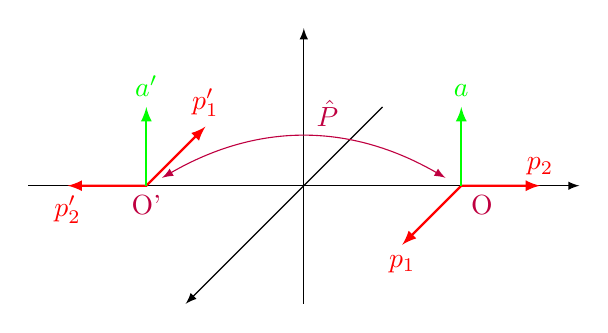
\begin{tikzpicture}
		%nodes
		\node at (2,0) (o1) [purple, anchor=north west] {O};
		\node at (-2,0) (o2) [purple, anchor=north] {O'};
		
		%lines
		\draw [->, -latex] (-3.5,0) -- (3.5,0);
		\draw [->, -latex] (0,-1.5) -- (0,2);
		\draw [->, -latex] (1,1) -- (-1.5, -1.5);
		%
		\draw [red, thick, <->, >=latex] (1.25,-0.75) node [below] {$p_1$} -- (o1.north west) -- (3,0) node [above] {$p_2$};
		\draw [red, thick, <->, >=latex] (-1.25,0.75) node [above] {$p_1^\prime$} -- (o2.north) -- (-3,0) node [below] {$p_2^\prime$};
		\draw [green, thick, ->, >=latex] (o1.north west) -- (2,1) node [above] {$a$};
		\draw [green, thick, ->, >=latex] (o2.north) -- (-2,1) node [above] {$a^\prime$};
		%
		\draw [purple] (1.8,0.1) edge [bend right, <->, >=latex] node [midway, above, xshift=0.3cm] {$\hat{P}$} (-1.8, 0.1);
	\end{tikzpicture}
	\caption{Die (gestrichenen und ungestrichenen) $p_1, p_2$--Vektoren sind die oben genannten Polar--Vektoren, die $a$--Vektoren die Axial--Vektoren.}
\end{figure}

\section{Anwendung auf die Teilchenphysik}
Offensichtlich ist die Parität abhängig von der Wahl des Ursprungs: beispielsweise kann man durch Verschiebung des Ursprungs um $\nicefrac{\pi}{2}$ eine Kosinusfunktion in eine Sinusfunktion umwandeln, was die Parität ändert. 

In der Teilchenphysik kann man trotzdem einem Teilchen eine \textbf{intrinsische Parität} zuweisen. Diese intrinsische Parität ist jene, die das Teilchen in dem System hat, in dem der Ursprung im geometrischen Mittelpunkt liegt (auch für mehrere Teilchen,für punktförmige Elementarteilchen etwas schwer vorstellbar; es handelt sich hierbei allerdings um ein eher theoretisches Konzept). 

Empirisch findet man, dass die Parität eines Systems eine multiplikative Erhaltungsgröße unter starker, elektromagnetischer und gravitativer Wechselwirkung ist, jedoch nicht unter schwacher Wechselwirkung. 

Um zu verstehen, was \textit{multiplikativ} hier bedeutet, betrachten wir die Parität eines 2--Teilchen--Systems aus Teilchen $\alpha$ und $\beta$, deren intrinsische Paritäten $\pi_\alpha,\ \pi_\beta$ bereits bekannt sind. Wir müssen hier annehmen, dass die Teilchen nicht verschränkt sind, sodass man ihre Wellenfunktion als Produkt schreiben kann. Da wir die intrinsische Parität des 2--Teilchen--Systems betrachten wollen, interessiert uns nun lediglich die Relativbewegung $\phi$ der Teilchen zueinander. Wir schreiben
\begin{equation}
	\psi_{\alpha \beta} \lp \vec{r}_\alpha ,\ \vec{r}_\beta \rp = \psi_\alpha \lp \vec{r}_\alpha \rp \psi_\beta \lp \vec{r}_\beta \rp \phi \lp \vec{r}_\alpha - \vec{r}_\beta\rp
\end{equation}
wobei $\psi_\alpha$ und $\psi_\beta$ die Einzelwellenfunktionen und $\phi$ die Relativbewegung beschreiben. 

Vom H--Atom wissen wir, dass sich (sofern das Potential der einzelnen Teilchen radialsymmetrisch ist, was (zumindest näherungsweise) in der Teilchenphysik immer der Fall ist) $\phi \lp \vec{r}_\alpha - \vec{r}_\beta\rp$ in Kugelflächenfunktionen entwickeln lässt. Wir können auch annehmen, dass $\phi \lp \vec{r}_\alpha - \vec{r}_\beta\rp$ eine konkrete Kugelflächenfunktion ist, da sonst (siehe H--Atom) bei geladenen Teilchen Dipolübergänge stattfinden, die als Resultat wieder eine konkrete Kugelflächenfunktion haben (Superpositionen von Kugelflächenfunktionen sind also zeitlich instabil). Somit folgt:
\begin{equation}
	\hat{P}\psi_{\alpha \beta} = \pi_\alpha \pi_\beta \cdot (-1)^\ell \psi_{\alpha \beta}
\end{equation}
Hier wird die Multiplikativität der Parität deutlich. Für Mehrteilchen--Systeme kann man diesen Separationsansatz iterieren. 

Es ist ersichtlich, dass nun dem Photon die Parität $\pi_\gamma = -1$ zuweisen muss, da beispielsweise bei einem Dipolübergang im H--Atom unter Abstrahlung eines Photons die Auswahlregel $\Delta \ell = \pm 1$ gilt, was die Parität des H--Atoms ändert, die elektromagnetische Wechselwirkung diese jedoch erhöht.

Man findet $\pi = -1$ für alle Eichbosonen. Für Nukleonen findet man $\pi_p = \pi_n = 1$. 

Darüber hinaus findet man für die Paritäten von Teilchen und Antiteilchen:
\begin{align*}
	\text{Fermionen: } \pi_F &= -\pi_{\ol{F}}\\
	\text{Bosonen: } \pi_B &= \pi_{\ol{B}}
\end{align*}

Bei unserer bisherigen Betrachtung des Zwei--Teilchen--Systems haben wir nur die ''Ortsparität'' berücksichtigt, jedoch trägt der Spinraum auch zur Gesamtparität bei: 

Annahme: beide Teilchen haben die gleiche Spinquantenzahl $s_\alpha = s_\beta$. Dann können sie entweder zu einem symmetrischen Triplett $(S=1)$ oder einem antisymmetrischen Singulett $(S=0)$ koppeln. Die Spinwellenfunktion liefert also den Eigenwert 
\begin{equation}
	\pi_\chi = (-1)^{s+1}
\end{equation}
Somit erhalten wir unter Berücksichtigung einer Spinwellenfunktion also
\begin{equation}
	\hat{P} \lp \psi_{\alpha \beta} \lp \vec{r}_\alpha ,\ \vec{r}_\beta \rp \chi_{\alpha \beta} \rp = \pi_\alpha \pi_\beta (-1)^{\ell + s + 1} \cdot \psi_{\alpha \beta} \chi_{\alpha \beta}
\end{equation}
Man benutzt $J^\pi$ als neue Größe, die gleichzeitig Gesamtdrehimpuls und Parität eines Teilchens charakterisiert. (Häufig findet man auch $S^\pi$, also nur Spin und Parität). Mesonen lassen sich dadurch wie folgt bezeichnen:
\begin{table}[H]
	\centering
	$
	\begin{array}{rl}
	\text{Skalarmesonen:} & J^\pi = 0^+ \\ 
	\text{pseudoskalare Mesonen:} & J^\pi = 0^- \\ 
	\text{(polare) Vektormesonen:} & J^\pi = 1^- \\ 
	\text{axiale/pseudo--Vektormesonen:}  & J^\pi = 1^+
	\end{array} 
	$
\end{table}



\end{document}